\documentclass[a4paper,11pt, oneside]{book}
%\documentclass[a4paper,twoside,11pt,titlepage]{book}
\usepackage{listings}
\usepackage[utf8]{inputenc}
\usepackage[spanish]{babel}

% \usepackage[style=list, number=none]{glossary} %
%\usepackage{titlesec}
%\usepackage{pailatino}

\decimalpoint
\usepackage{dcolumn}
\newcolumntype{.}{D{.}{\esperiod}{-1}}
\makeatletter
\addto\shorthandsspanish{\let\esperiod\es@period@code}
\makeatother


%\usepackage[chapter]{algorithm}
\RequirePackage{verbatim}
%\RequirePackage[Glenn]{fncychap}
\usepackage{fancyhdr}
\usepackage{graphicx}
\usepackage{afterpage}

\usepackage{longtable}

\usepackage[pdfborder={000}]{hyperref} %referencia

\usepackage{amsthm}
\usepackage{amsmath}
\usepackage{amssymb}


% ********************************************************************
% Re-usable information
% ********************************************************************
\newcommand{\myTitle}{Título del proyecto\xspace}
\newcommand{\myDegree}{Grado en ...\xspace}
\newcommand{\myName}{Nombre Apllido1 Apellido2 (alumno)\xspace}
\newcommand{\myProf}{Nombre Apllido1 Apellido2 (tutor1)\xspace}
\newcommand{\myOtherProf}{Nombre Apllido1 Apellido2 (tutor2)\xspace}
%\newcommand{\mySupervisor}{Put name here\xspace}
\newcommand{\myFaculty}{Escuela Técnica Superior de Ingenierías Informática y de
Telecomunicación\xspace}
\newcommand{\myFacultyShort}{E.T.S. de Ingenierías Informática y de
Telecomunicación\xspace}
\newcommand{\myDepartment}{Departamento de ...\xspace}
\newcommand{\myUni}{\protect{Universidad de Granada}\xspace}
\newcommand{\myLocation}{Granada\xspace}
\newcommand{\myTime}{\today\xspace}
\newcommand{\myVersion}{Version 0.1\xspace}



\hypersetup{
pdfauthor = {\myName (email (en) ugr (punto) es)},
pdftitle = {\myTitle},
pdfsubject = {},
pdfkeywords = {palabra_clave1, palabra_clave2, palabra_clave3, ...},
pdfcreator = {LaTeX con el paquete ....},
pdfproducer = {pdflatex}
}

%\hyphenation{}


%\usepackage{doxygen/doxygen}
%\usepackage{pdfpages}
\usepackage{url}
\usepackage{colortbl,longtable}
\usepackage[stable]{footmisc}
%\usepackage{index}

%\makeindex
%\usepackage[style=long, cols=2,border=plain,toc=true,number=none]{glossary}
% \makeglossary

% Definición de comandos que me son tiles:
%\renewcommand{\indexname}{Índice alfabético}
%\renewcommand{\glossaryname}{Glosario}

\pagestyle{fancy}
\fancyhf{}
\fancyhead[LO]{\leftmark}
\fancyhead[RE]{\rightmark}
\fancyhead[RO,LE]{\textbf{\thepage}}
\renewcommand{\chaptermark}[1]{}



\setlength{\headheight}{1.5\headheight}

\newcommand{\HRule}{\rule{\linewidth}{0.5mm}}
%Definimos los tipos teorema, ejemplo y definición podremos usar estos tipos
%simplemente poniendo \begin{teorema} \end{teorema} ...
\newtheorem{teorema}{Teorema}[chapter]
\newtheorem{ejemplo}{Ejemplo}[chapter]
\newtheorem{definicion}{Definición}[chapter]

\definecolor{gray97}{gray}{.97}
\definecolor{gray75}{gray}{.75}
\definecolor{gray45}{gray}{.45}
\definecolor{gray30}{gray}{.94}

\lstset{ frame=Ltb,
     framerule=0.5pt,
     aboveskip=0.5cm,
     framextopmargin=3pt,
     framexbottommargin=3pt,
     framexleftmargin=0.1cm,
     framesep=0pt,
     rulesep=.4pt,
     backgroundcolor=\color{gray97},
     rulesepcolor=\color{black},
     %
     stringstyle=\ttfamily,
     showstringspaces = false,
     basicstyle=\scriptsize\ttfamily,
     commentstyle=\color{gray45},
     keywordstyle=\bfseries,
     %
     numbers=left,
     numbersep=6pt,
     numberstyle=\tiny,
     numberfirstline = false,
     breaklines=true,
   }
 
% minimizar fragmentado de listados
\lstnewenvironment{listing}[1][]
   {\lstset{#1}\pagebreak[0]}{\pagebreak[0]}

\lstdefinestyle{CodigoC}
   {
	basicstyle=\scriptsize,
	frame=single,
	language=C,
	numbers=left
   }
\lstdefinestyle{CodigoC++}
   {
	basicstyle=\small,
	frame=single,
	backgroundcolor=\color{gray30},
	language=C++,
	numbers=left
   }

 
\lstdefinestyle{Consola}
   {basicstyle=\scriptsize\bf\ttfamily,
    backgroundcolor=\color{gray30},
    frame=single,
    numbers=none
   }


\newcommand{\bigrule}{\titlerule[0.5mm]}


%Para conseguir que en las páginas en blanco no ponga cabecerass
\makeatletter
\def\clearpage{%
  \ifvmode
    \ifnum \@dbltopnum =\m@ne
      \ifdim \pagetotal <\topskip
        \hbox{}
      \fi
    \fi
  \fi
  \newpage
  \thispagestyle{empty}
  \write\m@ne{}
  \vbox{}
  \penalty -\@Mi
}
\makeatother

\graphicspath{ {imagenes/} }

\usepackage{pdfpages}

\newtheorem{defi}{Definición}

\newtheorem{prop}{Proposición}


\begin{document}
\begin{titlepage}
 
 
\newlength{\centeroffset}
\setlength{\centeroffset}{-0.5\oddsidemargin}
\addtolength{\centeroffset}{0.5\evensidemargin}
\thispagestyle{empty}

\noindent\hspace*{\centeroffset}\begin{minipage}{\textwidth}

\centering

\includegraphics[width=0.9\textwidth]{imagenes/logo_ugr.jpg}\\[1.4cm]

\textsc{ \Large TRABAJO FIN DE GRADO\\[0.2cm]}
\textsc{ INGENIERÍA EN ...}\\[1cm]
% Upper part of the page
% 
% Title
{\Huge\bfseries Titulo del Proyecto\\
}
\noindent\rule[-1ex]{\textwidth}{3pt}\\[3.5ex]
{\large\bfseries Subtitulo del Proyecto}
\end{minipage}

\vspace{2.5cm}
\noindent\hspace*{\centeroffset}\begin{minipage}{\textwidth}
\centering

\textbf{Autor}\\ {Nombre Apellido1 Apellido2 (alumno)}\\[2.5ex]
\textbf{Directores}\\
{Nombre Apellido1 Apellido2 (tutor1)\\
Nombre Apellido1 Apellido2 (tutor2)}\\[2cm]

\includegraphics[width=0.3\textwidth]{imagenes/etsiit_logo.png}\\[0.1cm]
\textsc{Escuela Técnica Superior de Ingenierías Informática y de Telecomunicación}\\
\textsc{---}\\
Granada, mes de 201
\end{minipage}
%\addtolength{\textwidth}{\centeroffset}
%\vspace{\stretch{2}}
\end{titlepage}



\chapter*{}
%\thispagestyle{empty}
%\cleardoublepage

%\thispagestyle{empty}

\begin{titlepage}
 
 
\setlength{\centeroffset}{-0.5\oddsidemargin}
\addtolength{\centeroffset}{0.5\evensidemargin}
\thispagestyle{empty}

\noindent\hspace*{\centeroffset}\begin{minipage}{\textwidth}

\centering
%
\includegraphics[width=0.9\textwidth]{imagenes/logo_ugr.jpg}\\[1.4cm]

%\textsc{ \Large PROYECTO FIN DE CARRERA\\[0.2cm]}
%\textsc{ INGENIERÍA EN INFORMÁTICA}\\[1cm]
% Upper part of the page
% 

 \vspace{3.3cm}

%si el proyecto tiene logo poner aquí

\includegraphics{imagenes/logo.png} 
 \vspace{0.5cm}

% Title

{\Huge\bfseries Sistema de adaptación motora con entorno de realidad virtual\\
}
%\noindent\rule[-1ex]{\textwidth}{3pt}\\[3.5ex]
%{\large\bfseries Subtítulo del proyecto.\\[4cm]}
\end{minipage}

\vspace{2.5cm}
\noindent\hspace*{\centeroffset}\begin{minipage}{\textwidth}
\centering

\textbf{Autor}\\ {Nombre Apellido1 Apellido2 (alumno)}\\[2.5ex]
\textbf{Directores}\\
{Nombre Apellido1 Apellido2 (tutor1)\\
Nombre Apellido1 Apellido2 (tutor2)}\\[2cm]
%
\includegraphics[width=0.15\textwidth]{imagenes/tstc.png}\\[0.1cm]
%\textsc{Departamento de Teoría de la Señal, Telemática y Comunicaciones}\\
%\textsc{---}\\
%Granada, mes de 201
\end{minipage}
%\addtolength{\textwidth}{\centeroffset}
\vspace{\stretch{2}}

 
\end{titlepage}






\cleardoublepage
\thispagestyle{empty}

\begin{center}
{\large\bfseries Título del Proyecto: Subtítulo del proyecto}\\
\end{center}
\begin{center}
Nombre Apellido1 Apellido2 (alumno)\\
\end{center}

%\vspace{0.7cm}
\noindent{\textbf{Palabras clave}: palabra\_clave1, palabra\_clave2, palabra\_clave3, ......}\\

\vspace{0.7cm}
\noindent{\textbf{Resumen}}\\

Poner aquí el resumen.
\cleardoublepage


\thispagestyle{empty}


\begin{center}
{\large\bfseries Project Title: Project Subtitle}\\
\end{center}
\begin{center}
First name, Family name (student)\\
\end{center}

%\vspace{0.7cm}
\noindent{\textbf{Keywords}: Keyword1, Keyword2, Keyword3, ....}\\

\vspace{0.7cm}
\noindent{\textbf{Abstract}}\\

Write here the abstract in English.

\chapter*{}
\thispagestyle{empty}

\noindent\rule[-1ex]{\textwidth}{2pt}\\[4.5ex]

Yo, \textbf{Nombre Apellido1 Apellido2}, alumno de la titulación TITULACIÓN de la \textbf{Escuela Técnica Superior
de Ingenierías Informática y de Telecomunicación de la Universidad de Granada}, con DNI XXXXXXXXX, autorizo la
ubicación de la siguiente copia de mi Trabajo Fin de Grado en la biblioteca del centro para que pueda ser
consultada por las personas que lo deseen.

\vspace{6cm}

\noindent Fdo: Nombre Apellido1 Apellido2

\vspace{2cm}

\begin{flushright}
Granada a X de mes de 201 .
\end{flushright}


\chapter*{}
\thispagestyle{empty}

\noindent\rule[-1ex]{\textwidth}{2pt}\\[4.5ex]

D. \textbf{Nombre Apellido1 Apellido2 (tutor1)}, Profesor del Área de XXXX del Departamento YYYY de la Universidad de Granada.

\vspace{0.5cm}

D. \textbf{Nombre Apellido1 Apellido2 (tutor2)}, Profesor del Área de XXXX del Departamento YYYY de la Universidad de Granada.


\vspace{0.5cm}

\textbf{Informan:}

\vspace{0.5cm}

Que el presente trabajo, titulado \textit{\textbf{Título del proyecto, Subtítulo del proyecto}},
ha sido realizado bajo su supervisión por \textbf{Nombre Apellido1 Apellido2 (alumno)}, y autorizamos la defensa de dicho trabajo ante el tribunal
que corresponda.

\vspace{0.5cm}

Y para que conste, expiden y firman el presente informe en Granada a X de mes de 201 .

\vspace{1cm}

\textbf{Los directores:}

\vspace{5cm}

\noindent \textbf{Nombre Apellido1 Apellido2 (tutor1) \ \ \ \ \ Nombre Apellido1 Apellido2 (tutor2)}

\chapter*{Agradecimientos}
\thispagestyle{empty}

       \vspace{1cm}


Poner aquí agradecimientos...


%\frontmatter
%\tableofcontents
%\listoffigures
%\listoftables
%
%\mainmatter
%\setlength{\parskip}{5pt}

%\input{capitulos/01_Introduccion}
%
%\input{capitulos/02_EspecificacionRequisitos}
%
%\input{capitulos/03_Planificacion}
%
%\input{capitulos/04_Analisis}
%
%\input{capitulos/05_Diseno}
%
%\input{capitulos/06_Implementacion}
%
%\input{capitulos/07_Pruebas}
%
%\input{capitulos/08_Conclusiones}
%
%%\chapter{Conclusiones y Trabajos Futuros}
%
%
%%\nocite{*}
%\bibliography{bibliografia/bibliografia}\addcontentsline{toc}{chapter}{Bibliografía}
%\bibliographystyle{miunsrturl}
%
%\appendix
%\input{apendices/manual_usuario/manual_usuario}
%%\input{apendices/paper/paper}
%\input{glosario/entradas_glosario}
% \addcontentsline{toc}{chapter}{Glosario}
% \printglossary
\tableofcontents

\chapter{Introduccion}


\chapter{Objetivos}
\subsection{Experimento de referencia}
Para diseñar el experimento tomamos como referencia el artículo Cerebellar Contributions to Reach Adaptation and Learning Sensory Consequences of Action. En este artículos los investigadores llevan a cabo un experimento en el que se estudian dos tipos de aprendizaje de movimientos diferentes:  de modelo directo y de modelo inverso.

En el modelo inverso se asocia un objetivo con el comando motor necesario para alcanzarlo, mientras que en el modelo directo se asocia un comando motor con sus consecuencias sensoriales. La motivación del artículo es dar soporte a la teoría de que el cerebelo no está implicado en el aprendizaje del modelo inverso, lo que explicaría por qué algunos pacientes con daños en el cerebelo son capaces de realizar con éxito determinados tipos de movimientos.

Para ello llevaron a cabo una serie de experimentos enfocados en disociar estos dos tipos de modelos. 

Durante la prueba los individuos tuvieron que alcanzar con un brazo robot un objetivo que se proyectaba en una pantalla, mientras que se ocultaba su mano para que no tuvieran visión de ella, pero sí del brazo robot. 

En la primera fase (fase de referencia), aparecieron una serie de dianas en un ángulo de 45º, que el sujeto tenía que golpear con el brazo robot. Primero se realizaron 50 repeticiones en la que se mostraba el cursor sin perturbación (la posición que se mostraba era la posición real), y luego 25 repeticiones sin mostrar el cursor.

Después (sin mostrar ningún objetivo ni el cursor) sino que se pidió a los sujetos que realizaran un movimiento dentro del primer cuadrante de un círculo. Al terminar el movimiento y traer el brazo robot al centro los sujetos tenían que señalar con la mano izquierda dónde creían que la mano derecha había cruzado el círculo. Esto se repetió 25 veces.

Por último se presentó un objetivo en ángulos de [15°, 25°, 35°, 45°, 55°, 65°, 75°]. El feedback visual (la representación del cursor) se proporció solo en los objetivos en ángulo de 45º, por lo que se probaba la capacidad de generalización de los individuos.

En la segunda fase (fase de adaptación) el target objetivo fue siempre 45º, y a lo largo de las repeticiones fue incrementando una perturbación entre el movimiento realizado y la posición del cursor en la pantalla. 

En la última fase (fase de postadaptación) se probó la capacidad de generalización de los individuos aplicando una perturbación de 30º, mostrando solamente el target 45º.

El experimento fue llevado a cabo con 10 pacientes sanos y 10 pacientes con algún tipo de daño en el cerebelo.

\chapter{Planificacion y coste}


En este capítulo vamos a tratar la planificación que se hizo del proyecto, así como los costes derivados de este. También estudiaremos si estas estimaciones iniciales fueron correctas, y en caso contrario, cuál sería el impacto en el coste final.

\section{Fases del proyecto}
El proyecto ha sido desarrollado en cuatro fases: planificación del experimento, desarrollo de la aplicación, obtención de resultados mediante la utilización de la aplicación en distintos usuarios y análisis de los resultados obtenidos. 
\begin{enumerate}
	\item Planificación del experimento: en esta etapa se definió el experimento que íbamos a realizar, teniendo en cuenta contenido, fases de las que consistiría y grupos de población en los que íbamos a realizarlo.
	\item Desarrollo de la aplicación: esta etapa se dedicó a desarrollar la aplicación que se utilizaría después para la realización de los experimentos. A su vez esta etapa se dividió en tres subetapas:
	\begin{enumerate}
		\item Instalación de los paquetes necesarios para utilizar el dispositivo System 3D Touch.
		\item Desarrollo del código necesario para implementar la aplicación.
		\item Revisión del código para utilizar los parámetros idóneos. Esta etapa se realizó una vez acabada la primera prueba de realización del experimento.
	\end{enumerate}
	\item Obtencion de resultados: en esta etapa distintos usuarios llevaron a cabo el experimento planeado, haciendo uso de la aplicación implementada en la fase anterior.
	A su vez esta etapa se dividió en dos:
	\begin{enumerate}
		\item Fase de prueba, en la que se eligió a un primer grupo de sujetos para la realización del experimento, cada uno con un set de parámetros diferentes. Esta fase nos ayudó a decidir los parámetros que queríamos utilizar finalmente.
		\item Fase final, en la que se eligió a un segundo grupo de sujetos (ninguno de los cuales había participado en la fase de prueba) y se realizó el experimento con los parámetros que finalmente habíamos elegido.
		Estos resultados fueron los que se utilizaron para fase Análisis de los resultados.
	\end{enumerate}
		
	\item Analisis de los resultados: en esta etapa analizamos las graficas obtenidas con los datos de la etapa anterior, para así obtener conclusiones del experimento.
\end{enumerate}

Por tanto podemos decir que el proyecto ha seguido un modelo de ciclo de vida en cascada, en el que en algunas etapas ha habido realimentación,dado que la información conseguida en algunas etapas nos ha servido para modificar etapas anteriores. Este proceso puede verse reflejado en la Figura:

Por otro lado la toma de decisiones en las distintas fases se ha llevado a cabo mediante reuniones regulares (telemáticas y presenciales) y la comunicación mediante correo electrónico.

\section{Planificación del proyecto en tiempo}
El proyecto fue pensado para ser desarrollado entre los meses de septiembre y junio. La planificacion inicial fue:
\begin{itemize}
	\item Septiembre: planificación del experimento.
	\item De octubre a diciembre: desarrollo de la aplicación.
	\item De enero a marzo: obtención de resultados
	\item De marzo hasta mayo: análisis de resultados y redacción de la memoria.
\end{itemize}
La etapa mas larga fue de la del desarrollo de la aplicación pues es la que sustentaba todo el trabajo que podíamos realizar después. Por eso fue la que más carga de trabajo acumuló, y a la que más horas se le dedicó.

El reparto de horas puede verse en la siguiente grafica:
\begin{itemize}
	\item Planificación del experimento: 10 horas. 
	\item Desarrollo de la aplicación:
		\begin{itemize}
			\item Instalación del software y familarización con el: 35 horas
			\item Desarrollo del programa: 60 horas
		\end{itemize}
	\item Obtención de resultados: 40 horas
	\item Análisis de resultados:
	\item Total de horas: 
\end{itemize}
Por tanto, teniendo en cuenta que el salario medio de un profesional junior es de /Hora, el coste en personal seria de ....

Por otro lado tenemos que añadir el coste del dispositivo System3D Touch: ´ 

Por último, dado la necesidad de realizar el experimento en individuos externos al proyecto y teniendo en cuenta la duración media de este (45 minutos) decidimos ofrecer una compensación material a los individuos que se presentaran voluntarios, en concepto de coste de transporte. La compensación la hemos fijado en 5 euros por persona, y dado que necesitamos -- voluntarios ( -- para la fase de prueba y -- para la fase final), el coste adicional será de --- euros.

Por tanto el presupuesto final fue de -- euros, repartido como puede verse en la siguiente figura:


\chapter{Material}

\section{Touch}

Touch ha sido el dispositivo sobre el que se ha hecho la aplicación, y que se ha utilizado posteriormente para la realización del experimento.

Es un dispositivo háptico desarrollado por la empresa 3D Systems. Los dispositivos hápticos simulan respuestas táctiles, mediante las cuales podemos percibir objetos tridimensionales en un ambiente de realidad virtual.
Según la propia documentación de 3D Systems: "Touch es un dispositivo motorizado que aplica retroalimentación de fuerza a la mano del usuario, lo que le permite sentir objetos virtuales y producir sensaciones táctiles reales a medida que el usuario manipula los objetos 3D en la pantalla". Touch es utilizado en aplicaciones de control robótico, rehabilitación, medicina y cirugía, etc.

Foto Touch

\subsection{OpenHaptics}

OpenHaptics es un software para desarrolladores hápticos que permite crear aplicaciones que utilicen Touch. Está basado en la API de OpenGL y está disponible para Windows de 64 bits 10 y 11 y para Linux. 

OpenHaptics incluye varias APIs desarrolladas en C++, y viene con varios ejemplos de aplicaciones, una guía de usuario y dos guías para los desarrolladores: OpenHaptics Programmers Guide y OpenHaptics API Reference Guide. 




\chapter{Fundamentos matemáticos}['fundamentos']

Un proceso clave a la hora de desarrollar la aplicación ha sido trasladar las coordenadas obtenidas a través del dispositivo Touch a la pantalla del ordenador. De esta forma hemos podido obtener las trayectorias que cada sujeto ha realizado tal y como ellos las han visto reflejadas en la pantalla. 

Para explicar el proceso de transformación de coordenadas vamos a introducir previamente algunos conceptos matemáticos que necesitaremos después. Las transformaciones que aplicaremos incluyen traslaciones, rotaciones, escalados y proyecciones. Para estudiar estos movimientos introduciremos dos conceptos matemáticos muy importantes: las transformaciones afines y las proyecciones. Estos conceptos se basan en el estudio de la Geometría afín y proyectiva, que a su vez tienen una base en el Álgebra lineal. 


\section{Álgebra lineal, Geometría afín y Geometría Proyectiva}
% https://www.emis.de/journals/DM/v14-2/art6.pdf
Podemos encontrar los primeros antecedentes del álgebra lineal en el libro del Cálculo, escrito por el sacerdote egipcio Ahmés hacia el año 1650 a.C. En él se describen algunos problemas relacionados con la agricultura, que involucran sistemas de ecuaciones de primer grado. Los matemáticos babilonios, griegos, chinos e islámicos siguieron estudiando estos tipos de problemas, pero no fue hasta el siglo  XIX cuando Hamilton, Cayley y Grassmann introdujeron las nociones de vector y espacio vectorial, desarrollando gran parte de los conceptos que estudiaremos en este capítulo. En el año 1850 Sylvester introdujo el término matriz, y en 1858, en su libro Memoir on the theory of matrices, Cayley utiliza las matrices para explicar las transformaciones lineales.

La geometría afín surge con Euler y se consolida con Klein en 1872 mediante el Programa de Erlangen, un programa de investigación con el objetivo de proponer una solución a los problemas que la Geometría se enfrentaba en ese momento. Klein define la geometría afín como una generalización de la geometria asociada al álgebra lineal. El espacio afín se construye sobre el espacio vectorial, con la diferencia de que no tenemos un vector de referencia, lo que nos dará la capacidad de hacer traslaciones. A su vez Klein engloba la geometría afín dentro de la geometría proyectiva.

En el Programa de Erlangen, Klein también introduce el concepto de Grupo (un conjunto en el que hay definido una operación que cumple ciertas propiedades) en la Geometría. Para Klein cada Geometría es el estudio de las propiedades que no cambian al aplicar un tipo de transformaciones. Por ejemplo, el algebra lineal estudia las propiedades de los espacios al aplicar movimientos lineales (escalados, rotaciones sobre el origen), la geometría afín al aplicar movimientos afines (traslaciones) y la geometría proyectiva al aplicar movimientos proyectivos.

En este capítulo vamos a introducir primero el concepto de espacio vectorial para después definir el concepto de espacio afín. Sobre el espacio afín estudiaremos como representar los movimientos afines en forma de matrices, y el concepto de sistema de referencia y por último cómo realizar un cambio de un sistema de referencia a otro. Este último resultado será el que utilicemos a la hora de explicar las operaciones que hemos realizado hacer los cambios de sistemas de coordenadas.

Por último estudiaremos brevemente el espacio proyectivo para poder explicar la proyección en perspectiva que realizaremos a la hora de proyectar el movimiento del cursor del dispositivo Touch en la pantalla.
% https://www.ugr.es/~arobles/MatApl(CivilADE)/Tema5_beamer.pdf

% https://www.ugr.es/~fjlopez/_private/Geometria_III.pdf
 


\subsection{Álgebra lineal}

El Álgebra lineal estudia los conceptos de espacios vectoriales y sus trasformaciones lineales. En esta sección nuestro objetivo es definir el concepto de espacio vectorial, que utilizaremos para definir después el espacio afín. Para ello necesitamos definir previamente los conceptos de grupo, anillo y cuerpo. 

También introduciremos el concepto de Base en un espacio vectorial, para el que necesitaremos definir los conceptos de combinación lineal de vectores, vectores linealmente independientes y sistemas de generadores. Por último terminaremos la sección con una proposición que nos permitirá hacer cambios de base con los vectores.

\begin{defi}
	Sea $G$ un conjunto. Decimos que $(G,*)$ es un grupo si existe una operación o ley de composición interna:
	\begin{equation}
	*: GxG \rightarrow G
	(x,y) \mapsto x*y
	\end{equation}
	que cumpla las siguientes propiedades:
	\begin{enumerate}
		\item Asociativa: $ x*(y*z) = (x*y)*z$, $\forall x,y,z \in G$.
		\item Elemento neutro: $\exists e \in G)$ (elemento neutro) tal que $e*x = x*e = x$, $\forall x \in G$.
		\item Elemento simétrico. $\forall x \in G$, $\exists \bar{x} \in G$ (elemento simétrico de $x$) tal que $x*\bar{x} = \bar{x}*x= e$.
	\end{enumerate}
	Si además cumple:
	\begin{itemize}
		\item Conmutativa: $x*y = y*x$, $\forall x,y \in G$.
	\end{itemize}
	diremos que el grupo es abeliano.
\end{defi}
\begin{defi}
	Diremos que $(A, +, *)$ es un anillo si verifica:
	\begin{enumerate}
	\item $(A, +)$ es un grupo conmutativo.	
	\item $(A, *)$ verifica la propiedad asociativa.
	\item $(A, +, *)$ verifica la propiedad distributiva de la suma respecto al producto, esto es,
	\begin{equation}
	x*(y+z) = x*y +x*z 
	(y+z)*x = y*x + z*x
	\end{equation}
	para todo $x,y,z \in A$.
	\end{enumerate}
	Un anillo unitario no trivial es un anillo cuyo producto tiene elemento neutro distinto de cero.
\end{defi}
\begin{defi}
	Un cuerpo $(K, +, *)$ es un anillo unitario no trivial en el que el producto verifica la propiedad elemento simétrico. El cuerpo es conmutativo si el producto $*$ verifica la propiedad conmutativa.
\end{defi}
\begin{defi}
	Sea $(K, +, *)$ un cuerpo conmutativo. Un espacio vectorial sobre $(K, +, *)$ es una terna $(V, +, *K)$ formada por un conjunto $V$ dotado de una operación (ley de composición interna) en $V$,
	\begin{equation}
	+ : V x V \rightarrow V
	\end{equation}
	y una aplicación
	\begin{equation}
	* : K x V \rightarrow V
	\end{equation}
	o ley de composición externa de $K$ sobre $V$ tales que:
	\begin{enumerate}
	\item $(V, +)$ es un grupo conmutativo. Esto es, la operación $+$ en $V$, que asocia a cada par $(u,v) \in V x V$ un único $u+v \in V$, verifica las propiedades de grupo abeliano.
	\item La ley de composición externa $* : K x V \rightarrow V$, que asocia a cada $a \in K$ y cada $
	v \in V$ un único vector que denotaremos $a * v \in V$, verifica las propiedades:
	\begin{enumerate}
		\item Pseudoasociativa: $(a * b)*v = a*(b*v)$ para todo $a,b \in K$ y todo $v \in V$.
		\item Unimodular: $1*v = v$, para todo $v \in V$, donde 1 es el elemento neutro de $(K\{0\},*)$.
		\item Distributiva respecto de la suma en $K:(a+b)*v=a*v+b*v$, para cualesquiera $a,b \in K$ y $v \in V$.
		\item Distributiva respecto de la suma en $V: a*(u+v) = a*u+a*v$, para todo $a \in K$ y cualesquiera $u,v \in V$.
	\end{enumerate}
	\end{enumerate}
\end{defi}
\begin{defi}
	Sea $V(K)$ un espacio vectorial y $S = \{v_1,...,v_m\}$ una familia finita no vacía de vectores de $V$. Una combinación lineal de $S$ es cualquier vector de $V$ obtenido al multiplicar cada $v_i$ por un escalar $a_i \in K$ y después sumar los vectores resultantes:
	\begin{equation}
	a_1*v_1+...+a_m*v_m, donde a_i \in K \forall i = 1,...,m.
	\end{equation}
	Llamaremos $L(S)$ al subconjunto de V formado por los vectores obtenidos como combinación lineal de $S$:
	\begin{equation}
	L(S) = L(v_1,...,v_m) = \{a_1*v_1+...+a_m*v_m : a_i \in K, \forall i = 1,...m\}.
	\end{equation}
\end{defi}
\begin{defi}
	Sea $V(K)$ y $S = \{v_1,...,v_m\}$ una familia finita no vacía de vectores de $V$. Diremos que $S$ es linealmente independiente si se cumple:
	\begin{enumerate}
		\item Caso $m=1$: $v_1 \neq 0$.
		\item Caso $m \geq 2$: ningún vector de $S$ es combinación lineal de los restantes vectores de $S$, esto es, $v_i \notin L(S -\{v_i\})$, para cada $i=1,...,m$.
	\end{enumerate}
\end{defi}
\begin{defi}
	Sea $V(K)$ y sea $S \subset V$ un conjunto no vacío. Se dice que $S$ es un sistema de generadores si $V = L(S)$. Esto equivale a que todo vector de $V$ se expresa como combinación lineal finita de vectores de $S$, es decir, para cada $v \in V$, existen $m \in N$, vectores $v_1,...,v_m \in S$ y escalares $a_1,...,a_m \in K$, tales que $v = a_1*v_1+...+a_m*v_m$.
\end{defi}
\begin{defi}
	Sea $V$ un espacio vectorial sobre un cuerpo $K$. Una base de $V$ es una familia no vacía $B \subset V$ tal que $B$ es un sistema de generadores de $V$ y $B$ es linealmente independiente.
\end{defi}
\begin{defi}
	Supongamos $V$ un espacio vectorial sobre un cuerpo $K$ con $dim_k(V) = n$. Tomamos dos bases $B = \{v_1,...,v_n\}$ y $B' = \{v_1,...,v_n\}$ de $V$ y $ v \in V$. La matriz de cambio de base de $B$ a $B'$ es la matriz que denotaremos $M(I, B' \leftarrow B)$ cuya columna j-ésima contiene las coordenadas del vector $v_j$ de $B$ respecto de $B'$. Lo simbolizamos así:
	\begin{equation}
	M(I, B' \leftarrow B) = ((v_1)_{B'} | ... |(v_n)_{B'})
	\end{equation}
\end{defi}
\begin{prop}
	En las condiciones anteriores se tiene que:
	\begin{equation}
	v_{B'} = M(I, B' \leftarrow B)* v_B
	\end{equation}
\end{prop}
\begin{proof}
	Supongamos que:
	\begin{equation}
	v_j = a_{1j}*v'_1 +...+ a_{nj}*v'_n, para cada j = 1,...,n
	\end{equation}
	De esta forma la j-ésima columna de $M(I, B' \leftarrow B)$  contiene exactamente a los escalares $a_{ij}$ con $i=1,...,n$. Supongamos también que:
	\begin{equation}
	v = x_1*v_1+...+x_n*v_n
	\end{equation}
	es decir, $v_B$ contiene a los escalares $x_i$ con $i=1,...,n$. Buscamos expresar $v$ como combinación lineal de $B'$. Sustituyendo la primera ecuación en la segunda tenemos la igualdad:
	\begin{equation}
	\begin{split}
	v &= x_1*(a_{11}*v'_{1}+...+a_{n1}*v'_n)+...+x_n*(a_{1n}*v'_1+...+a_{nn}*v'_n) \\
	 &= 
	 (a_{11}*x_1+...+a_{1n}*x_n)*v'_1 +...+(a_{n1}*x_1+...+a_{nn}*x_n)*v'_n
	 \end{split}
	\end{equation}
	que expresa $v$ como combinación lineal de $B'$. Esto significa que los coeficientes de la combinación lineal anterior son las coordenadas de $v$ respecto de $B'$. Por definición de producto de matrices, la entrada i-ésima de $v_{B'}$ es el producto de la fila i-ésima de $M(I, B' \leftarrow B)$ con el vector columna $v_B$.
\end{proof}

\subsection{Geometría afín}

En esta sección vamos a definir la base teórica para realizar cambios de sistemas de coordenadas. Las transformaciones que aplicaremos son escalados, giros y traslaciones, y para ello definiremos el concepto de espacio afín. Después definiremos el concepto de sistema de referencia afín para terminar demostrando la fórmula del cambio de sistema de referencia, que es la que utilizaremos en el apartado práctico.

\begin{defi}
	Un espacio afín es una tripleta $(A, V, \rightarrow)$ donde
	\begin{itemize}
		\item $A$ es un conjunto no vacío
		\item $V \equiv (V, +, *\Re)$ es un espacio vectorial real
		\item $\rightarrow$ : $A x A \rightarrow V$, $(p,q) \mapsto \overrightarrow{pq}$, es una aplicación satisfaciendo
		$A_1 : \overrightarrow{pq} + \overrightarrow{qr} = \overrightarrow{pr}$.
		$A_2$ : $\forall p \in A$, $\forall v \in V$ , $\exists! q \in A : \overrightarrow{pq} = v$.
	\end{itemize}
	Al espacio vectorial $V$ lo vamos a denotar como $\overrightarrow{A}$. La dimensión de $A$ es la de $\overrightarrow{A}$.
\end{defi}
\begin{defi}
	Una colección de puntos $\{p_0,...,p_k\}, k \in K$, en un espacio afín $A$ se dice afínmente independiente si los vectores $\{\overrightarrow{p_0p_1},...,\overrightarrow{p_0p_k}\}$ son linealmente independientes si
	\begin{equation}
	dim<{p_0,p_1,...,p_k}> = k
	\end{equation}
\end{defi}
\begin{defi}
	Dado un espacio afín $A$ con dim $A = n \in N$, un sistema de referencia $R$ en $A$ es un sistema ordenado $\{p_0, ..., p_n\}$ de $n+1$ puntos afínmente independientes o equivalentemente satisfaciendo:
	\begin{equation}
	<\{p_0,p_1,...,p_n\}> = A
	\end{equation}
	Al punto $p_0$ se le llama origen del sistema, y a la base ordenada $B = \{\overrightarrow{p_0p_1}, ..., \overrightarrow{p_0p_n}\}$ de $\overrightarrow{A}$ se le llama base asociada de las direcciones de $R$.
	Si $B = \{v_1,...,v_n\}$ es una base ordenada de $\overrightarrow{A}$ y $p_0 \in A$, el sistema ordenado de puntos
	\begin{equation}
	R = \{p_0, p_0+v_1, ..., p_0+v_n\}
	\end{equation}
	es un sistema de referencia de $A$ con origen $p_0$ y base asociada de direcciones $B$. Por tanto, y de forma alternativa, podríamos definir un sistema de referencia como un par
	\begin{equation}
	R = \{p_0, B\}
	\end{equation}
	donde $p_0$ es un punto de $A$ y $B$ una base ordenada de $\overrightarrow{A}$.
\end{defi}

\begin{defi}
	Sea $A$ un espacio afín, y consideremos un sistema de referencia afín $R = \{p_0,...,p_n\} \equiv \{p_0, B\}$, donde
	$B = \{\overrightarrow{p_0p_1},...,\overrightarrow{p_0p_n}\}$. La aplicación biyectiva
	\begin{equation}
	\Phi_R : A \rightarrow \Re^n, \phi_R = \phi_B \circ F_{p_0}
	\end{equation}
	es conocida como la aplicación asignación de coordenadas (con notación columna) en el sistema de referencia R. De forma simplificada escribiremos
	\begin{equation}
	p_R := \Phi_B(F_{p_0}(p)) \equiv (\overrightarrow{p_0p})_B \in \Re^n, 
	\end{equation}
	y diremos que $p_R$ son las coordenadas de p $\in$ $A$ en $R$.
\end{defi}
\begin{prop}
	Sea $A$ un espacio afín y $R = \{p_0,...,p_n\} \equiv \{p_0,B\}$ un sistema de referencia afín, donde $B = \{\overrightarrow{p_0p_1},...,\overrightarrow{p_0p_n}\}$. Entonces
	\begin{enumerate}
		\item $(p+v)_R = p_R + v_B$
		\item $(\overrightarrow{pq})_B = q_R - p_R$
	\end{enumerate}
\end{prop}
\begin{proof}
	Usando la definición anterior y que $\Phi_B$ es lineal, tenemos que:
	\begin{equation}
	(p+v)_R = (\overrightarrow{p_0(p+v)})_B = (\overrightarrow{p_0p}+v)_B = (\overrightarrow{p_0p})_B +v_B = p_R +v_B
	\end{equation}
	lo que prueba $(i)$. Análogamente,
	\begin{equation}
	q_R - p_R = (\overrightarrow{p_0q})_B - (\overrightarrow{p_0p})_B = (\overrightarrow{p_0q} - \overrightarrow{p_0p})_B = (\overrightarrow{pp_0}+\overrightarrow{p_0q})_B = (\overrightarrow{pq})_B
	\end{equation}
	lo que prueba $(ii)$.
\end{proof}
\begin{prop}
		La fórmula del cambio de sistema de referencia es:
	\begin{equation}
		p_{R'} = (p_0)_{R'} + M(Id_{\overrightarrow{A}}, B, B')p_R
	\end{equation}
\end{prop}
\begin{proof}
	Utilizando la proposición y la definición anterior:
	\begin{equation}
	p_{R'} = (p_0 + \overrightarrow{p_0p})_{R'} = (p_0)_{R'} + (\overrightarrow{p_{0}p})_{B'} = (p_0)_{R'} + M(Id_{\overrightarrow{A}}, B, B') * (\overrightarrow{p_0p})_B,
	\end{equation}
	y por tanto,
	\begin{equation}
	p_{R'} = (p_0)_{R'} + M(Id_{\overrightarrow{A}}, B, B')p_R
	\end{equation}
\end{proof}

\begin{prop}
La ecuación anterior puede escribirse de forma compacta utilizando una única matriz de orden $n+1$. Esta matriz es de la forma:
\begin{equation}
M(Id_A, R, R') := 
\begin{pmatrix}
M(Id, B, B') & (p_0)_{R'} \\
0 			 & 1 \\
\end{pmatrix}
\end{equation}
Podemos escribir la fórmula del cambio de sistema de referencia como:
\begin{equation}
\begin{pmatrix}
1 \\
p_{R'}
\end{pmatrix}
 = M(Id_A, R, R')*\begin{pmatrix}
 1 \\
 p_R
 \end{pmatrix}
\end{equation}
\end{prop}
\begin{proof}
	Para demostrarlo...
\end{proof}

Por tanto hemos puesto la base para conocer las coordenadas en un sistema de referencia $R'$ de un punto $p \in A$ a partir de las coordenadas de $p$ en otro sistema de referencia $R'$ teniendo:
\begin{itemize}
	\item Coordenadas en $R'$ del origen $p_0$ de $R$.
	\item Matriz del cambio de base en $\overrightarrow{A}$ de la base $B$ de las direcciones de $R$ a la base $B'$ de las direcciones de $R'$.
\end{itemize}

\subsection{Espacio Proyectivo}

En esta sección vamos a definir los principios básicos del espacio proyectivo, que utilizaremos como base teórica para poder explicar después la proyección en perspectiva que aplicaremos a las coordenadas para representarlas en la pantalla del ordenador.


Antes de definir el espacio proyectivo necesitamos dos conceptos previos: relación de equivalencia y espacio cociente.

\begin{defi}
	R es una relación de equivalencia sobre K si:
	\begin{enumerate}
	\item $\forall x \in K$	: $xRx$
	\item $\forall x,y \in K$: $xRy \Rightarrow yRx$
	\item $\forall x,y,x \in K$: $xRy ^ yRz \Rightarrow xRz$.
	\end{enumerate}
\end{defi}

\begin{defi}
	Dado X un espacio vectorial y R una relación de equivalencia, el espacio cociente generado por ella está definido por:
	\begin{equation}
		X \setminus \backsim := \{[x]: x \in X\}
	\end{equation}
\end{defi}



Nota: A partir de ahora llamaremos $E^* = E \setminus \{0\}$.
\begin{defi}
	Sea $E$ un espacio vectorial con $dim E=n+1$, llamamos $P(E)$, espacio proyectivo, al espacio cociente
	\begin{equation}
		P(E) = E^* / \backsim
	\end{equation}
	siendo la relación de equivalencia:
	\begin{equation}
		v \backsim w \Leftrightarrow v = \lambda w \textup{ para algún } \lambda \in R^* 
	\end{equation}
	Llamaremos $[v] \in P(E)$ a la clase de equivalencia de $v \in E^*$, es decir, al punto de $P(E)$ determinado por la recta vectorial genereada por $v$:
	\begin{equation}
		[v] = L(\{v\})^* := \{\lambda v: \lambda \in R^*\}
	\end{equation}
	Por lo que podemos decir que los puntos de $P(E)$ son rectas vectoriales de $E$.
\end{defi}

El concepto de coordenadas en $P(E)$ es diferente, ya que no hay un concepto natural de base. Es por eso por lo que se introducen las coordenadas homogéneas.
\begin{defi}
	Las coordenadas homogéneas de un punto $p \in P(E)$ en la base $B = \{v_0,v_1,...,v_n\}$ de $E$ las definimos como:
	\begin{equation}
		p_b = \{\lambda v_B: \lambda \in R^*\}
	\end{equation}
	donde $v_B \in (R^{n+1})$ son las coordenadas en $B$ de cualquier vector $v$ no nulo tal que $[v] = p$. Si $v_B = (x_0,v_1,...,x_n)$, escribiremos:
	\begin{equation}
		p_B = (x_0:x_1:...:x_n) := \{\lambda(x_0,x_1,...,x_n): \lambda \in R^*\}
	\end{equation}
\end{defi}

Nuestro objetivo ahora es poder relacionar el espacio euclidiano $R^n$ con el proyectivo $P^n$. 

Podemos ver que todo espacio afín $A$ se puede ver como un hiperplano afín que no pasa por el origen en un espacio vectorial $E$ de una dimensión mayor. Esto lo podemos conseguir fijando un origen $e_0 \in A$ y definiendo $E = R \times A$:
\begin{equation}
	A \ni p \longleftrightarrow (1, \overrightarrow{e_0p}) \in \{1\}\times\overrightarrow{A} \ \subset E^*
\end{equation}
De esta forma llevamos el origen $e_0$ al punto $(1,0)$. 

Siguiendo este razonamiento podemos definir el hiperplano $A \subseteq R^{n+1}$ donde $\{x_0 = 1\}$ como:
\begin{equation}
	A = \{1\} \times R^n \subseteq R^{n+1}
\end{equation}
e identificar $R^n$ con $A$ de la siguiente forma:
\begin{equation}
	R^n \rightarrow A \textup{,  } (x_1,...,x_n) \mapsto (1,x_1,...,x_n)
\end{equation}

El embebimiento canónico de $R^n$ en $P^n = P(R^{n+1})$ queda:
\begin{equation}
	e: R^n \rightarrow A \textup{,   } e((x_1,...,x_n)) = (1:x_1:...:x_n)
\end{equation}

Por tanto la relación entre el espacio euclidiano $R^n$ y el proyectivo $P^n$ es:
\begin{equation}
	R^n \textup{ } \underrightarrow{e} \textup{ } P^n \setminus R^n_{\infty}\textup{,     } (x_1,...,x_n) \longmapsto (1:x_1:...:x_n)
\end{equation}
\begin{equation}
	P^n \setminus R^n_{\infty} \textup{ }   \underrightarrow{e^{-1}} \textup{ }R^n \textup{,     } (x_0:x_1:...:x_n) \longmapsto (\frac{x_1}{x_0},...,\frac{x_n}{x_0})
\end{equation}
donde $R^n_{\infty} = \{(0:x_1:...:x_n) : (x_1:...:x_n) \in  P^{n-1}\}$

Esto último es lo que utilizaremos para hacer la proyección que necesitamos para transformar las coordenadas del dispositivo a la pantalla.


\section{Aplicaciones en informática gráfica}

El problema que queremos resolver es: teniendo las coordenadas que nos proporciona el dispositivo Touch, ¿qué transformaciones tenemos que hacer para obtener las coordenadas del cursor de Touch en la pantalla?


Para ello tenemos que entender los distintos sistemas de coordenadas que utiliza OpenGL y el cauce de transformaciones que aplica a los objetos para representarlos en la pantalla. Podemos verlo representado en la siguiente imagen:
\\

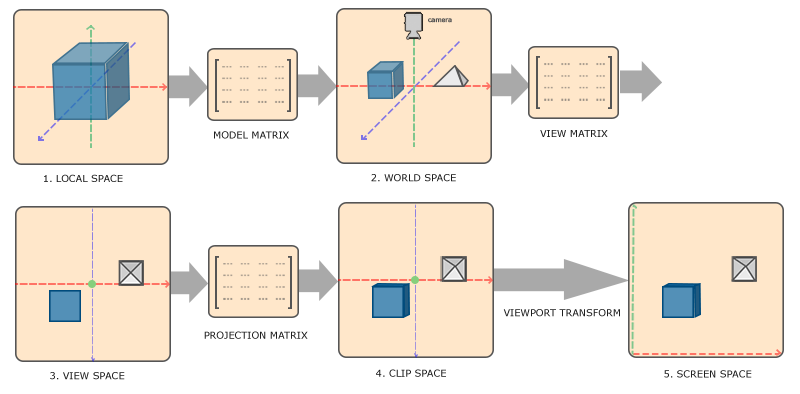
\includegraphics[scale=0.4]{coordinate_systems}



Podemos ver que OpenGL utiliza diferentes sistemas de coordenadas:
\begin{itemize}
	\item Coordenadas locales (local coordinates): coordenadas del objeto relativas a su propio origen.
	\item Coordenadas del mundo (world coordinates): coordenadas del objeto relativas a un origen global del sistema, donde están situados los demás objetos.
	\item Coordenadas de vista (view coordinates): coordenadas del objeto desde el punto de vista de la cámara.
	\item Coordenadas de recorte (clip coordinates): coordenadas respecto a un cubo virtual desde el que determinaremos qué vértices se verán en la pantalla. El cubo tiene dimensiones $[-1,1]\cdot[-1,1]\cdot[-1,1]$.
	\item Coordenadas de pantalla (screen coordinates): coordenadas del objeto tal y como lo vemos representado en la pantalla. El origen de las coordenadas de pantalla está situado en la en la esquina inferior izquierda.
\end{itemize} 

Además vamos a introducir un sistema de coordenadas que nos permitirá situarnos respecto a los targets que representaremos en la pantalla. Queremos centrar el origen de este sistema de coordenadas en el target de referencia y situar los demás targets en una circunferencia de radio $2$. Estas serán las coordenadas que utilizaremos para dibujar las trayectorias y las llamaremos coordenadas finales.

\begin{itemize}
	\item Coordenadas finales: en este sistema de coordenadas el origen es el punto inicial de la aplicación, y los demás puntos están situados en la circunferencia de radio 2.
\end{itemize}

%https://learnopengl.com/Getting-started/Coordinate-Systems
%https://programmerclick.com/article/7153348621/


Las coordenadas que Touch nos proporciona están en el sistema de referencia local. Por lo tanto nuestro objetivo es estudiar las transformaciones que se realizan para, a partir de esas coordenadas, obtener las coordenadas finales.

Como hemos estudiado en la sección anterior las transformaciones entre sistemas de referencia se realizan a través de la multiplicación de las matrices de cambio de sistema de referencia. Estas matrices en OpenGL tienen los siguientes nombres:

\begin{itemize}
	\item Matriz modelo (model matrix): matriz de cambio del sistema de referencia local al sistema de referencia del mundo.
	\item Matriz de vista (view matrix): matriz de cambio del sistema de referencia del mundo al sistema de referencia de vista.
	\item Matriz de proyección (projection matrix): matriz de cambio del sistema de referencia de vista al sistema de referencia de recorte.
	\item Viewport: matriz de cambio de sistema de referencia de recorte al sistema de referencia de pantalla.
\end{itemize}

 OpenGL combina la matriz modelo y la matriz vista en una matriz llamada modelview. Además, como hemos introducido otro sistema de referencia, tenemos que definir otra matriz para pasar de sistemas de coordenadas de pantalla a sistema de coordenadas finales. Esta matriz la llamaremos la matriz final.

Por tanto el diagrama que vamos a seguir es:

\begin{enumerate}
	\item Aplicamos las transformaciones de OpenGL, es decir:
	\begin{equation}
	C. Locales \rightarrow C. Vista \rightarrow C.Recorte \rightarrow C.Pantalla
	\end{equation}
	\item Aplicamos la matriz final para obtener las coordenadas finales
	\begin{equation}
		C.Pantalla \rightarrow C.Finales
	\end{equation}
\end{enumerate}


Vamos a definir ahora la notación que vamos a utilizar para representar los distintos sistemas de coordenadas:

\begin{itemize}
	\item $R$: sistema de coordenadas locales
	\item $R'$: sistema de coordenadas de vista
	\item $R''$: sistema de coordenadas de recorte
	\item $R'''$: sistema de coordenadas de pantalla
	\item $R''''$: sistema de coordenadas de pantalla
\end{itemize}

Y las correspondientes matrices de cambio de coordenadas son:

\begin{itemize}
	\item $(Id, R', R)$: modelview
	\item $(Id, R'', R')$: projection
	\item $(Id, R''', R'')$: viewport
	\item $(Id, R'''', R''')$: matriz final
\end{itemize}

En las siguientes secciones vamos a tomar un punto $v$ en el sistema de coordenadas $R$ y vamos a estudiar las transformaciones que OpenGL le aplica para obtener el punto en el sistema de coordenadas $R'''$. Para ello, utilizando el la función $glGetDoublev$ de $Gl.h$, obtendremos las matrices que OpenGL aplica en cada paso y las analizaremos utilizando los conceptos que hemos definido previamente.

%glGetDoublev Gl.h.


\subsection{Paso de coordenadas locales a coordenadas de vista}

OpenGL aplica la transformación de coordenadas locales a coordenadas de vista utilizando una única matriz: la matriz modelview. En este paso vamos a tomar $p_R$ y queremos obtener $p_{R'}$ utilizando $(Id, R', R)$, que será la matriz modelview.
La matriz modelview que utiliza la aplicación es:
$$(Id, R', R) = \begin{pmatrix}
	1 & 0 & 0& 0 \\
	0 & 1&0&0 \\
	0&0&1&-6.49 \\
	0&0&0&1
\end{pmatrix}$$
y el cambio de sistemas de coordenadas será:
$$p_{R'} = \begin{pmatrix}
	1 & 0 & 0& 0 \\
	0 & 1&0&0 \\
	0&0&1&-6.49 \\
	0&0&0&1
\end{pmatrix}*p_{R}$$
Como hemos explicado antes, esto es una notación abreviada de:
\begin{equation}
p_{R'} = 
\begin{pmatrix}
0\\
0\\
-6.49
\end{pmatrix}
+
\begin{pmatrix}
1&0&0 \\
0&1&0\\
0&0&1
\end{pmatrix}
*p_R
\end{equation}
Por tanto lo que estamos haciendo es una transformación afín, en concreto una traslación del origen de sistema de coordenadas en el eje z.

\subsection{Paso de coordenadas de vista a coordenadas de recorte}
Ahora vamos a hacer el cambio de sistemas de coordenadas de vista al sistema de coordenadas de recorte.

El objetivo de este cambio de sistema de coordenadas es transformar la región visible del espacio en un cubo $[-1,1]\cdot[-1,1]\cdot[-1,1]$, utilizando una proyección en perspectiva, como podemos ver en la siquiente imagen.
\\

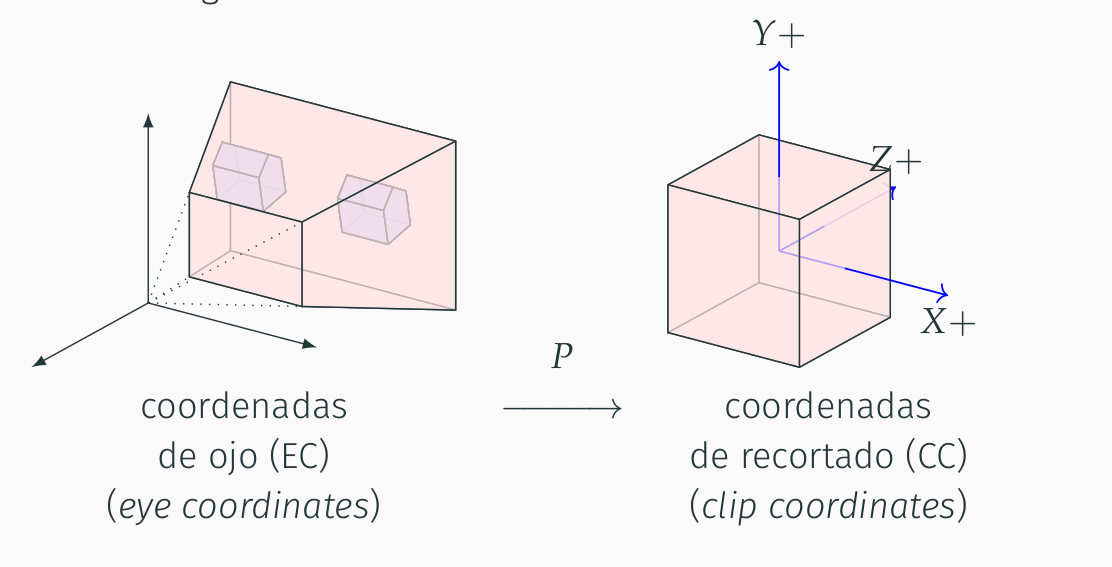
\includegraphics[scale=0.2]{cubo}

La notación que utilizaremos será:
\\

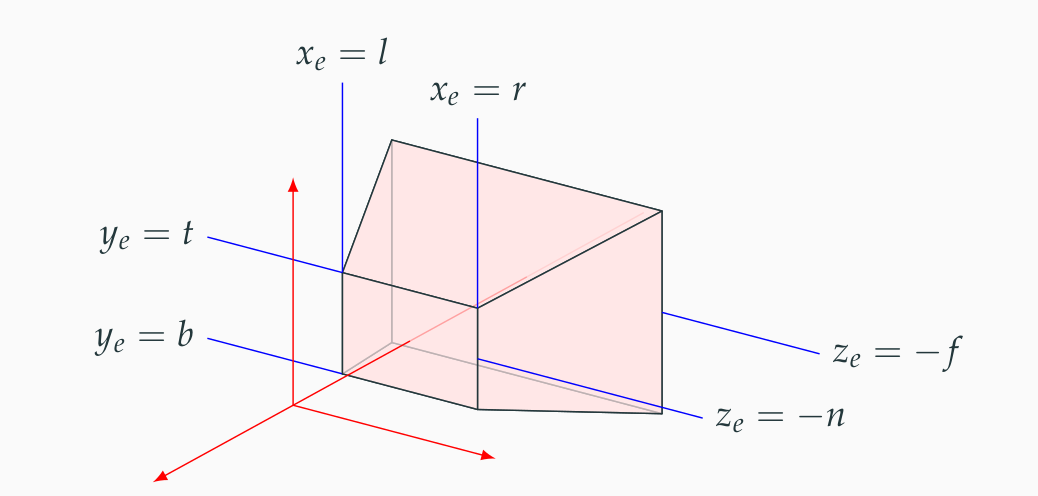
\includegraphics[scale=0.2]{notacion}
\\

Para ello primero calcularemos la proyección en el eje $z$ de las coordenadas $x,y$. Como hemos estudiado antes, para obtener la proyección sobre el plano euclídeo tenemos que dividir por la última coordenada. En este caso como además queremos que los puntos se proyecten sobre el valor $z=-n$, en lugar de $z=1$, tendremos que multiplicar por $-n$. Si tenemos $(x',y',z')$ en el sistema de referencia $R'$.
\begin{equation}
x''_e = x'\cdot\frac{-n}{z'}
\end{equation}
\begin{equation}
y''_e = y'\cdot\frac{-n}{z'}
\end{equation}
\begin{equation}
z''_e = z'\cdot\frac{-n}{z'} = -n
\end{equation}

Tenemos que $(x''_e,y''_e)$ sería el punto que obtendríamos sobre el plano euclídeo (plano situado sobre $z=-n$).

Sabemos ahora que $x''_e \in [l,v]$ y $y''_e \in [b,t]$. Para conseguir que ambos estén en el intervalo $[-1,1]$ tenemos que aplicar un escalado y una traslación. 

\begin{equation}
x'' = 2\cdot(\frac{x''_e-l}{r-l})-1
\end{equation}
\begin{equation}
y'' = 2\cdot(\frac{x''_e-b}{t-b})-1
\end{equation}

Sustituyendo en las ecuaciones anteriores, y utilizando las constantes $a_0,a_1, b_0, b_1$.
\begin{equation}
x'' = \frac{a_0 \cdot x'}{-z'} -a_1 = \frac{a_0 \cdot x'+a_1 \cdot z'}{-z'}
\end{equation}
\begin{equation}
y'' = \frac{b_0 \cdot y'}{-z'} -b_1 = \frac{b_0 \cdot y'+b_1 \cdot z'}{-z'}
\end{equation}
donde
\begin{equation}
a_0 = \frac{2n}{r-l}
\end{equation}
\begin{equation}
a_1 = \frac{r+l}{r-l}
\end{equation}
\begin{equation}
b_0 = \frac{2n}{t-b}
\end{equation}
\begin{equation}
b_1 = \frac{t+b}{t-b}
\end{equation}

Estas transformaciones no se pueden implementar en una matriz, ya que no son lineales (aparece un denominador). Para poder escribirlo en forma de matriz vamos a hacer uso de una coordenada adicional, que nos va a servir para guardar el término no lineal, en este caso $-z$:

\begin{equation}
x'' = a_0 \cdot x'+a_1 \cdot z'
\end{equation}
\begin{equation}
y'' = b_0 \cdot y'+b_1 \cdot z'
\end{equation}
\begin{equation}
w'' = -z'
\end{equation}

La matriz que transforma las coordenadas $(x',y',z')$ en las coordenadas $(x'',y'',w'')$ es:

$$\begin{pmatrix}
x''\\
y''\\
w
\end{pmatrix}=
\begin{pmatrix}
	a_0 & 0&a_1\\
	0&b_0&b_1\\
	0&0&-1
\end{pmatrix}*
\begin{pmatrix}
x'\\
y'\\
z'
\end{pmatrix}
$$


De esta forma, una vez aplicadas las transformaciones afines, podemos obtener las coordenadas del plano de la siguiente forma:
\begin{equation}
(x'',y'',w'') -> (\frac{x''}{w''}, \frac{y''}{w''})
\end{equation}


Con este procedimiento tendríamos calculadas las coordenadas $x,y$ de pantalla. Sin embargo OpenGL utiliza EPO (eliminación de partes ocultas) para dibujar los objetos en la pantalla, lo que significa que tenemos que guardar información sobre la profundidad, para saber qué puntos están más cerca de otros y así poder superponerlos adecuadamente. 

Para ello vamos a  utilizar una función lineal en la coordenada $z$, que lleve el rango $[-f,-n]$ a $[-1,1]$:

\begin{equation}
z'' = \frac{c_0\cdot z'+c_1}{-z'}
\end{equation}
donde
\begin{equation}
c_0 = \frac{n+f}{n-f}
\end{equation}
\begin{equation}
c_1 = \frac{2fn}{n-f}
\end{equation}

Incluyendo ahora esta nueva ecuación en la matriz anterior tenemos:

$$\begin{pmatrix}
x''\\
y''\\
z'' \\
w
\end{pmatrix}=
\begin{pmatrix}
a_0 & 0&a_1&0\\
0&b_0&b_1&0\\
0&0&c_0&c_1\\
0&0&-1&0
\end{pmatrix}*
\begin{pmatrix}
x'\\
y'\\
z'\\
1
\end{pmatrix}
$$

Este sería el cambio de sistema de coordenadas que estábamos buscando. Comprobamos ahora que la matriz de proyección que utilizamos en la aplicación tiene esta forma (la obtenemos con glGetDoublev):

$$\begin{pmatrix}
2.74748 & 0&0&0\\
0&2.74748 &0&0\\
0&0&-3.74748&-22.5922\\
0&0&-1&0
\end{pmatrix}$$

La matriz tiene la estructura que hemos definido, siendo:
$$a_0 = 2.74748;
a_1 = 0;
b_0 = 2.74748;
b_1 = 0;
c_0 = -3.74748;
c_1 = -22.5922;
$$

\subsection{Paso de coordenadas de recorte a coordenadas de pantalla}
Por lo tanto ya tenemos las coordenadas de recorte y ahora vamos a calcular las coordenadas de pantalla. Las coordenadas de pantalla se expresan en píxeles y nos dicen cuál va a ser la representación en la pantalla del ordenador del objeto.

Los parámetros de la ventana que vamos a utilizar son:
\begin{itemize}
	\item $x_l, y_b$: número de columna y fila que ocupa la esquina inferior izquierda de la ventana.
	\item $w,h$: anchura y altura de la ventana
	\item $n_d, f_d$: rango de valores de z, siendo $n_d$ la profundidad más cercana al observador y $f_d$ la más lejana.
\end{itemize}
Podemos verlo en la siguiente imagen:
\\

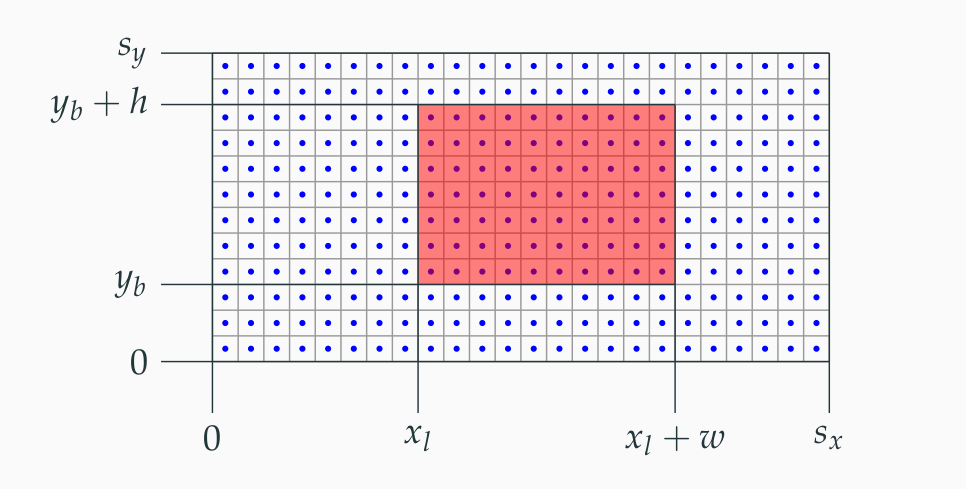
\includegraphics[scale=0.2]{viewport}
\\

Las condiciones que tenemos que realizar para pasar de coordenadas de recorte a coordenadas de pantalla son:
\begin{itemize}
	\item en el eje de coordenadas $x$ tenemos que llevar el intervalo $[-1,1]$ al intervalo $[x_l, x_l+w]$.
	\item en el eje de coordenadas $y$ tenemos que llevar el intervalo $[-1,1]$ al intervalo $[y_b, y_b+h]$.
	\item en el eje de coordenadas $z$ tenemos que llevar el intervalo $[-1,1]$ al intervalo $[n, f]$.
\end{itemize}

Por tanto las transformaciones que tenemos que aplicar son:
\begin{equation}
x''' = (x''+1)\cdot \frac{w}{2}+a
\end{equation}
\begin{equation}
y''' = (y''+1)\cdot \frac{h}{2}+b
\end{equation}
\begin{equation}
z''' = (z''+1)\cdot \frac{f-n}{2}+n
\end{equation}

Las cuales las podemos representar en la matriz:
\begin{equation}
\begin{pmatrix}
x'''\\
y'''\\
z'''\\
1
\end{pmatrix} =
\begin{pmatrix}
\frac{w}{2} &0&0&\frac{w}{2}+a\\
0&\frac{h}{2} &0&\frac{h}{2}+b\\
0&0&\frac{f-n}{2} & \frac{f+n}{2}\\
0&0&0&1
\end{pmatrix}
*\begin{pmatrix}
x''\\
y''\\
z''\\
1
\end{pmatrix}
\end{equation}

En la que podemos ver que estamos aplicando un escalado $[\frac{w}{2}, \frac{h}{2}, \frac{f-n}{2}]$ y una traslación $[\frac{w}{2}+a, \frac{h}{2}+b, \frac{f+n}{2}]$. OpenGL toma $f=1$ y $n=0$ y guarda los valores de $(a,b,w,h)$ en el vector viewport. 

\subsection{Paso de coordenadas de pantalla a coordenadas finales}´

Por último tenemos que pasar de coordenadas de pantalla a las coordenadas  finales que son las que utilizaremos para dibujar las trayectorias.

Para ello vamos a realizar dos transformaciones afines:
\begin{itemize}
	\item El origen de nuestro sistema de coordenadas queremos que esté en el target de referencia. Al haber hecho una proyección para pasar de sistemas de coordenadas locales a sistemas de coordenadas de pantalla sabemos que un punto en las coordenadas de pantalla corresponde a una recta en las coordenadas de dispositivo. En concreto el punto de referencia que estamos buscando es la recta que pasa por el punto $(0,0)$ en las coordenadas de dispositivo. Por tanto, utilizando solo un punto de esa recta (el $(0,0)$) podemos saber cómo se representa en la pantalla. Aplicamos las transformaciones que hemos estudiado antes (modelo-vista-proyección-viewport) al punto $(0,0)$ y nos da $(250,250)$. Por lo tanto la traslación que estamos buscando es la que lleva el punto $(250,250)$ al punto $(0,0)$, es decir:
	\begin{equation}
	x'''' = x'''-250
	\end{equation}
	\begin{equation}
	y''' = y'''-250
	\end{equation}
	\item Por otro lado queremos que en nuestro sistema de referencia los puntos estén situados en la circunferencia de radio 2, por lo tanto tenemos que aplicar un escalado. Para saber el escalado que tenemos que hacer aplicamos la transformación modelo-vista-proyección-viewport al punto objetivo $(2\cdot \cos(\pi/4),2\cdot \sin(\pi/4))$. Después calculamos la distancia del punto que nos ha dado al punto origen, y dividimos la distancia de nuestro punto origen a nuestro punto objetivo entre esa distancia. El resultado es $0.00945962$, que será el factor de escala.
\end{itemize}
Por último vamos a representar estas transformaciones afines en forma de matriz:

\begin{equation}
\begin{pmatrix}
x''''\\
y''''\\
1
\end{pmatrix} =
\begin{pmatrix}
0.0009 &0&-250\\
0&0.0009&-250\\
0&0&1 \\
\end{pmatrix}
*\begin{pmatrix}
x'''\\
y'''\\
1
\end{pmatrix}
\end{equation}

Y de esta forma ya tenemos todas las transformaciones que vamos a hacer para obtener las coordenadas con las que dibujaremos las trayectorias.


\chapter{Desarrollo del proyecto}




En este capítulo vamos a hablar de cómo se han desarrollado las diferentes fases del proyecto así como de los resultados obtenidos.

\section{Planificación del experimento}

En esta fase del proyecto decidimos cuál iba a ser la forma que iba a tener el experimento que posteriormente íbamos a realizar.

Desde el primer momento sabíamos que el objetivo era tener una aplicación en la que aparecieran una serie de puntos en la pantalla, y en la que el usuario tuviera que mover el cursor de un punto a otro haciendo movimientos balísticos. Posteriormente queríamos ser capaces de guardar la trayectoria de los movimientos realizados para poder analizarlas después.



\subsection{Diseño de nuestro experimento}

Dado que el objetivo del proyecto era probar el funcionamiento de System3D Touch en este tipo de experimentos, y no disponiendo de otros dispositivos complementarios, decidimos que el experimento consistiera en la aparición en pantalla de una serie de puntos sobre los que el sujeto debería situar el cursor.

Primero tendemos un punto de referencia en el centro, y cuando el sujeto se haya posado sobre él, desaparece este y aparece otro sobre una circunferencia alrededor del punto de referencia, en ángulos de 0, pi/4, pi/2, 3pi/4, pi, 5/4pi, 3pi/2, 7pi/4. Al haber situado el cursor sobre el punto objetivo, o al haber terminado el tiempo límite, el punto objetivo desaparece y aparece otra vez el punto de referencia, volviendo a empezar otra iteración. Las trayectorias que nos interesan son las del punto de referencia al punto objetivo.

Tenemos además cinco fases, en las que cambian las condiciones en como se comporta 3DSystem Touch:

\begin{itemize}
	\item Fase de adaptación: en esta fase solo se muestra el cursor sin ningún punto objetivo. El sujeto es libre para hacer cualquier tipo de movimiento. Esta fase sirve para que el sujeto se adapte a la utilización del dispositivo, así como para que tenga en cuenta las condiciones en las que el dispositivo no funciona correctamente, como cuando se acerca o se aleja en profundidad.
	\item Fase inicial, sin ninguna perturbación y mostrando el cursor.
	\item Segunda fase, en la que se muestra el cursor y se aplica una fuerza constante en la dirección x, en sentido negativo.
	\item Tercera fase, en la que no se aplica ninguna fuerza y se oculta el cursor en los movimientos desde el punto de referencia al punto objetivo. Al terminar el movimiento se vuelve a mostrar el cursor para volver al punto de referencia.
	\item Cuarta fase, en la que se aplica la misma fuerza de la segunda fase y se oculta el cursor siguiendo lo explicado en la tercera fase.
\end{itemize}

Los parámetros que teníamos que elegir eran:
\begin{itemize}
	\item Número de repeticiones por fase. Dado que la realización del experimento requiere de movimientos del brazo durante un periodo de tiempo moderado, teníamos que encontrar un acuerdo entre tener un número suficiente de repeticiones por punto objetivo y que el experimento no fuese demasiado exigente para los sujetos. Es por eso por lo que en la fase de prueba probamos diferentes configuraciones con sujetos de diferentes edades, desde 20 a 90 años. Finalmente elegimos tener 80 repeticiones por fase, para así tener 10 repeticiones por punto. Habría que tener en cuenta que en el caso de finalmente realizar el experimento con personas mayores de 80 años, sería recomendable bajar el número de repeticiones.
	\item Tiempo para la realización del movimiento. Este es un parámetro clave a la hora de diseñar el experimento, pues queríamos que los sujetos estuviesen obligados a hacer movimientos balísticos. Por lo tanto teníamos que encontrar un balance entre tener tiempo suficiente para que pudiesen alcanzar el punto y la obligación de que esos movimientos fuesen rápidos. Aquí también encontramos grandes diferencias en los resultados de personas jóvenes y más mayores, pero finalmente decidimos utilizar un tiempo de ..., con el que, una vez pasado un periodo de aprendizaje, todos los sujetos fueron capaces de alcanzar en ese tiempo el punto objetivo.
	\item Número y disposición de los puntos objetivos. Hicimos pruebas con diferentes sujetos con 8 puntos (como hemos mencionado arriba), 4 puntos (0, pi/2, pi, 4pi/3) y 2 puntos (0, pi). Pensamos que el experimento más interesante era con 8 puntos, pues así podíamos estudiar las diferencias en el aprendizaje de movimientos cuando hay que mover el cursor en un solo eje (los puntso 0, pi/2, pi, 4pi/3) a cuando hay que moverlo en dos ejes a la vez (pi/4, 3pi/4, 5/4pi, 7pi/4). En todo caso, y en relación con la dificultad en realizar un número grande de iteraciones en personas mayores, podría estudiarse el caso de reducir el número de puntos para así poder reducir a su vez el número de iteraciones.
	\item Disposición de los puntos objetivos siguiendo un orden o de forma aleatoria.
\end{itemize}

Otra decisión que tomamos fue la del criterio para considerar que un movimiento es correcto. En primer lugar pensamos que el criterio fuera que el sujeto pasase el cursor por encima del punto objetivo, de forma similar a como hacen en "Cerebellar Contributions to Reach Adaptation and Learning Sensory Consequences of Action". Después pensamos que sería interesante estudiar también, no solo que los sujetos realizaran el movimiento en la dirección correcta, sino con la distancia correcta. Por eso, para que el movimiento se considere correcto, el sujeto debe situar durante ... segundos el cursor encima del punto. Hicimos lo mismo a la hora de situar el cursor dentro del punto de referencia, e iniciar así el movimiento. Esto fue debido a que, en una pequeña demo inicial vimos que, si lo hacíamos solo con pasar el cursor sobre el punto de referencia, todos los movimientos empezaban con un desplazamiento en sentido contrario, el correspondiente al movimiento de volver al punto de referencia. De esta forma el sujeto está obligado a pararse dentro del punto inicial e iniciar el movimiento desde ahí.

También introdujimos un sonido cuando el movimiento no se ha realizado de forma correcta. Esto sirve de feedback al usuario, para saber cuando el movimiento se ha realizado correctamente y cuando no. 

Como hemos mencionado llevamos a cabo dos tandas de experimentos: una primera fase de prueba, para decidir los parámetros que íbamos a utilizar; y una segunda fase final para poder obtener resultados.

Uno de los requisitos era que en cada una de las fases tuviésemos representación de individuos de distintas edades, para no tener un sesgo a la hora de implementarla y obtener resultados. Teniendo en cuenta esto, y la disponibilidad de personas que teníamos a nuestro alrededor, los sujetos elegidos fueron:

\begin{tabular}{l l | l l}
	\multicolumn{2}{ c }{Fase 1} & \multicolumn{2}{ c }{Fase 2} \\ 
	Sexo & Edad & Sexo & Edad\\\hline 
	
	Mujer & 23 & Mujer & 20 \\
	Mujer & 24  & Mujer & 22\\
	Hombre & 53 & Hombre & 60\\
	Mujer & 52 & Hombre & 50 \\
	Hombre & 62  & Hombre & 60\\
	Mujer & 60 & Mujer & 59\\
	Hombre & 90 \\
	Mujer & 90 \\
\end{tabular} 

Como se puede comprobar, en la segunda fase la muestra de individuos fue similar a la primera, salvo porque no tuvimos individuos mayores de 80 años. Esto fue debido en parte a la poca disponibilidad que teníamos de individuos de edad más avanzada, y en parte a que decidimos realizar el experimento en unas condiciones que les eran menos favorables, con demasiadas repeticiones. Ninguno de los sujetos del experimento tenían un problema cerebral reconocido, por lo que podemos suponer que eran individuos sanos. No pudimos probar el experimento en individuos con problemas en el cerebelo, como hubiese sido lo ideal, por falta de disponibilidad.

\section{Desarrollo de la aplicación}

El objetivo de esta fase es desarrollar una aplicación sobre la que llevar a cabo el experimento diseñado en la fase de planificación, y también una forma de analizar los resultados que tengamos al realizar el experimento. Es decir, queremos tener como resultado:
\begin{itemize}
	\item Una aplicación diseñada para ejecutarse desde el ordenador, pues necesitamos utilizar a su vez el dispositivo Touch. \\
	Dicha aplicación debe tener:
	\begin{itemize}
		\item Un menú de selección para poder elegir entre los 5 modos de uso: libre, sin fuerza, con fuerza, sin fuerza y sin cursor y con fuerza y sin cursor.
		\item Al elegir el modo (salvo eligiendo el modo libre) debe aparecer una tarea que tendrá que realizarse un número determinado de iteraciones y que consistirá en:
		\begin{enumerate}
			\item Aparece el target de referencia, en la posición 0 (el centro).
			\item Al parar el cursor sobre el target de referencia este desaparece y aparece en su lugar un target situado sobre la circunferencia de radio 2 y centro el target de referencia. El nuevo target puede aparecer en cualquiera de las 8 posiciones: $\{0, \frac{\pi}{4}, \frac{\pi}{2}, \frac{3\pi}{4}, \pi, \frac{5\pi}{4}, \frac{3\pi}{2}, \frac{7\pi}{4}\}$
			\item Al parar el cursor sobre el target objetivo este desaparece y vuelve a aparecer el target de referencia.
		\end{enumerate}
		\item Se deben poder guardar las trayectorias y los tiempos del target de referencia al target objetivo. Cada una de las 4 fases se guardaŕa en un fichero csv diferente.
	\end{itemize}
	\item Un script de python que lea los ficheros csv generados al realizar el experimento y genere gráficas con los resultados en cada una de las fases de:
	\begin{itemize}
		\item Errores (distancia al target objetivo) en cada iteración. Por un lado queremos tener una gráfica con todos los errores de la fase, y por otro separados según el target objetivo.
		\item Tiempo transcurrido al realizar el movimiento. Al igual que con los errores, por fase y por target objetivo dentro de la fase.
		\item Distancia y velocidad al punto objetivo a través del tiempo, en cada uno de los ejes. Separado por targets objetivos.
	\end{itemize}
\end{itemize}


La fase del desarrollo de la aplicación tuvo tres partes: instalación del software necesario, implementación del código y revisión del código una vez elegidos los parámetros.

\subsection{Instalación del software de OpenHaptics}

La primera decisión que tuvimos que tomar fue si instalar el software de OpenHaptics en una máquina Ubuntu, o en una máquina Windows. Aunque en un principio la opción inicial fue instalarlo en Ubuntu 20.04, después de una prueba nos dimos cuenta de que Windows soportaba mejor la interfaz gráfica necesaria para llevarlo a cabo. Por tanto procedimos a realizar la instalación en Windows.

Los paquetes utilizados pueden encontrarse \href{https://support.3dsystems.com/s/article/OpenHaptics-for-Windows-Developer-Edition-v35?language=en\_US}{aquí}. Tenemos que instalar las \href{https://s3.amazonaws.com/dl.3dsystems.com/binaries/Sensable/OH/3.5/OpenHaptics_Developer_Edition_v3.5.0.zip}{librerías de OpenHaptics} y los \href{https://s3.amazonaws.com/dl.3dsystems.com/binaries/Sensable/driver/Touch_Device_Driver_2023.1.4.exe}{drivers de Touch}.
El toolkit de OpenHaptics necesita ciertos requerimientos hardware:
\begin{itemize}
	\item Procesador : 
	\begin{itemize}
		\item Intel i5 / i7, 5ª Generación o mayor 
		\item CPU mínimo 2.5 GHz de frecuencia.
		\item RAM 4 GB.
	\end{itemize}
	\item Tarjeta gráfica de mínimo 256 MB VRAM .
	\item Espacio de disco 512 MB.
	\item Resolución de pantalla 1280 x 800 (mínimo).
\end{itemize}
y software:
\begin{itemize}
	\item Sistema Operativo 64-bit Windows 7, 8.1, y 10
\end{itemize}

Tenemos tres documentos que nos servirán de ayuda para instalar y desarrollar utilizando OpenHaptics:
\begin{itemize}
	\item OpenHaptics Installation Guide: guía de instalación del toolkit de OpenHaptics.
	\item Programmer’s Guide: guía que explica la arquitectura de OpenHaptics, cómo funciona y lo que se puede hacer. Hay ejemplos de código, una explicación de cómo configurar Visual Studio para trabajar con la librería y una visión general de las tres APIs: QuickHaptics, HLAPI y HDAPI.
	\item API Reference Guide: contiene documentación sobre las funciones de QuickHaptics, HLAPI y HDAPI.
\end{itemize}

Las librerías de OpenHaptics están en c++, por lo tanto será el lenguaje de programación que utilizaremos. Las tres APIs que incluye son, como hemos comentado antes:
\begin{itemize}
	\item QuickHaptics: permite escribir rápido y fácilmente nuevas aplicaciones hápticas, o añadir funcionalidades hápticas a aplicaciones ya existentes.  
	\item HDAPI: provee un acceso a bajo nivel al dispositivo háptico, lo que permite a los programadores controlar las fuerzas que se pueden aplicar. 
	\item HLAPI: provee un acceso a alto nivel, similar a la API de OpenGL. Permite la reutilización de código de OpenGL.
\end{itemize}
En la siguiente imagen podemos ver cómo se relacionan las tres APIs:
\\
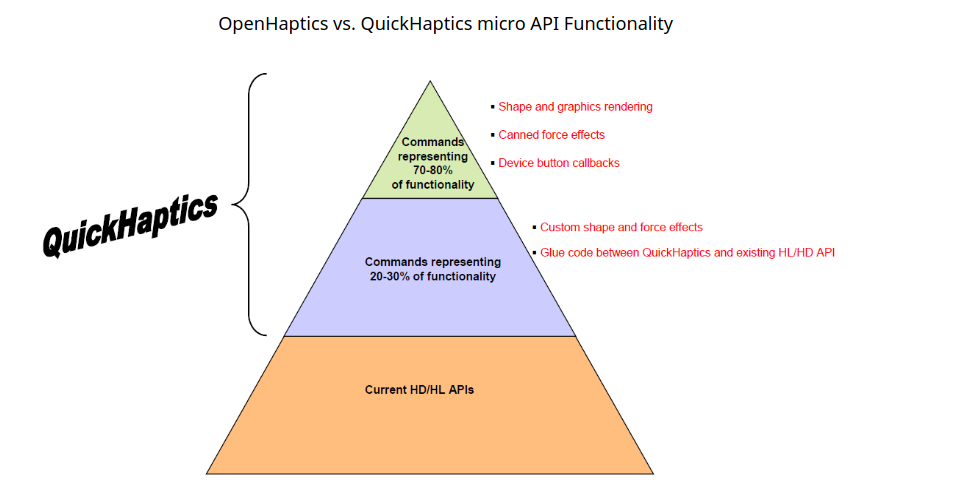
\includegraphics[scale=0.4]{OPENHAPTICS}
\\

En nuestro caso utilizaremos HDAPI, pues necesitamos controlar la fuerza que le aplicamos al dispositivo. También utilizaremos la biblioteca GLUT, una biblioteca de utilidades de OpenGL que nos permite manejar ventanas y representaciones gráficas.

\subsection{Implementación del codigo}

La estructura de un programa que utilice OpenHaptics es la siguiente: 


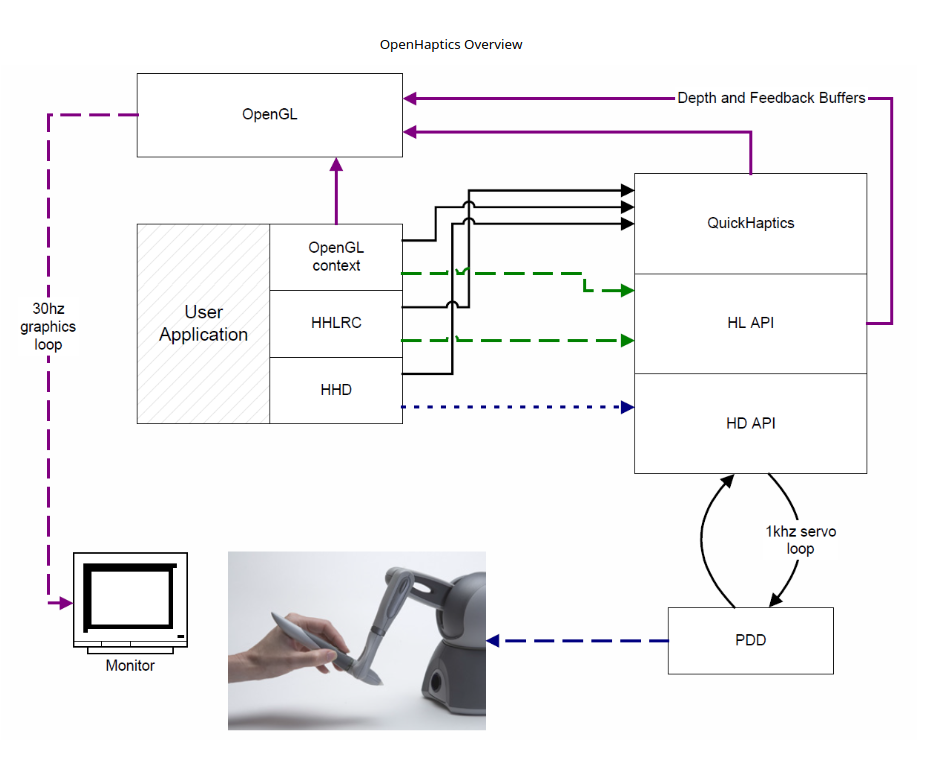
\includegraphics[scale=0.4]{estructura}

Como podemos ver tenemos dos bucles: el bucle gráfico y el servo loop.

El servo loop se usa para controlar las fuerzas que se mandan al dispositivo háptico. Para mantener un feedback consistente este bucle debe ejecutarse al menos a una frecuencia de 1000Hz, por lo que se ejecuta en una hebra diferente, con prioridad máxima. Para inicializar el servoloop utilizamos la función de HDAPI hdStartScheduler(). Se debe llamar una vez que se han inicializado las rutinas del dispositivo y se han añadido las callbacks asíncronas del scheduler. Una vez inicializado el servoloop empiezan a ejecutarse las callbacks que hemos definido, en cada iteración del bucle.

El bucle gráfico se ejecuta en una hebra diferente, y dado que el ojo humano no es capaz de procesar tantas imágenes por segundo, la frecuencia del bucle será menor, en concreto de 30Hz. El bucle gráfico se encarga de actualizar la representación gráfica, según los eventos que ocurran. Para inicializar el bucle gráfico utilizamos la función de GLUT glutMainLoop(). Una vez inicializado el bucle gráfico se llamarán en cada iteración a las callbacks que hayamos definido.

Dado que la frecuencia a la que se ejecutan los dos bucles es diferente, podemos tener problemas a la hora de que la hebra gráfica pida información a la hebra háptica sobre el estado del dispositivo. Para que el estado del dispositivo sea consistente se utiliza el scheduler, que provee sincronización entre las dos hebras.

Las callbacks del servoloop pueden ser síncronas o asíncronas. Las callbacks síncronas se usan principalmente para tener una instantánea del estado del dispositivo. Las callbacks síncronas solo devuelven el control de la hebra una vez terminadas, por lo que la aplicación tiene que esperar a que la función se haya terminado. Las callbacks asíncronas, por el contrario, devuelven el control justo cuando son programadas, por lo que la aplicación puede seguir ejecutándose. Son adecuadas para representar un efecto háptico, pues pueden perdurar en el tiempo, ya que en cada iteración se aplicará el efecto de la callback al dispositivo.

Las callbacks pueden devolver dos tipos de valores: HD\_CALLBACK\_DONE y HD\_CALLBACK\_CONTINUE. Las callbacks con return code DONE no volverán a ser ejecutadas en el bucle del servoloop hasta que vuelvan a ser programadas. Por el contrario, las callbacks con return code CONTINUE se vuelven a programar para la próxima iteración del bucle, hasta que explícitamente se especifique que se desprograme.

En nuestro caso las callbacks del servoloop son:
\begin{itemize}
	\item beginUpdateCallback: callback asíncrona, con return code CONTINUE. Se programa al inicializar el dispositivo háptivo y es la callback principal de la hebra háptica.  Actualiza el estado del dispositivo háptivo y escribe en el fichero csv las coordenadas del dispositivo (en caso de que se haya empezado el movimiento de ir desde el target de referencia al target objetivo, a lo que nos referiremos con que se ha inicializado la acción). 
	
	Dependiendo del momento de:
	\begin{itemize}
		\item Si la acción se ha inicializado comprueba el tiempo que ha transcurrido desde que se empezó la acción: si ha superado el tiempo límite programa la callback actionFinished.
		\item Si el cursor está en contacto con el punto de referencia, no se ha inicializado la acción y no estamos en la fase libre del experimento: comprueba si el cursor ha estado parado el tiempo necesario sobre el punto de referencia, si es así programa la callback actionInitialized.\\
		\item Si el cursor está en contacto con el target objetivo en esa iteración, la acción se ha inicializado y no estamos en la fase libre del experimento: si el cursor ha estado parado el tiempo necesario sobre el target objetivo se programa la callback actionFinished.
	\end{itemize}
	
	\item setDeviceTransformationCallback: callback síncrona, con return code DONE. Se programa al actualizar las transformaciones de coordenadas y calcula las transformaciones que hay que realizar.
	
	\item forceCallback: callback asíncrona, con return code CONTINUE. Se programa en la callback actionInitialized y aplica la fuerza que hemos configurado al dispositivo. 
	
	\item clearForceCallback: callback asíncrona, con return code CONTINUE. Se programa en la callback actionFinished y elimina la fuerza que se había aplicado antes, poniendo el vector fuerza nuevamente a 0. 
	
	\item actionInitialized: callback asíncrona, con return code DONE. Se programa en la callback beginUpdateCallback y sus funciones son:
	\begin{itemize}
		\item Oculta el target de referencia.
		\item Calcula el siguiente target objetivo y lo hace visible.
		\item Si estamos en algunas de las fases en las que se aplica fuerza al dispositivo, programa la callback forceCallback. 
		\item Inicializa el tiempo de inicio de acción.
		\item Si estamos en alguna de las fases en las que se oculta el cursor, hace el cursor no visible.
	\end{itemize}
	
	\item actionFinished: callback asíncrona con return code DONE. Se programa en la callback beginUpdateCallback y sus funciones son:
	\begin{itemize}
		\item Oculta el target objetivo.
		\item Muestra el target de referencia.
		\item Programa la callback clearForceCallback.
		\item Muestra el cursor.
		\item Si se han terminado las iteraciones diseñadas para la fase, selecciona la fase libre del experimento.
	\end{itemize}
\end{itemize}
Y las del bucle gráfico:
\begin{itemize}
	\item glutDisplayFunc: callback que se utiliza para actualizar la vista. En esta callback actualizamos el estado del dispositivo, capturando el último estado del servoloop. También dibujamos la escena, según el modo del menú que se haya elegido. 
	
	\item glutReshapeFunc: callback para actualizar las dimensiones de la ventana. También se actualiza la posición de la cámara.
	
	\item glutIdleFunc: callback para mandar una petición de redibujar la ventana.	
\end{itemize}

Vamos a hablar ahora del main y de las dos clases más importantes de la aplicación: HapticDeviceManager y PointManager.

\subsubsection{Main}

Las funciones del main son:
\begin{itemize}
	\item Inicializar la librería de GLUT: lo hacemos con la función glutInit().
	\item Crear y definir las dimensiones de la pantalla y el modo de visualización: glutCreateWindow(), glutInitDisplayMode() y glutInitWindowSize().
	\item Definir las callbacks que actualizarán el entorno gráfico: glutDisplayFunc, glutReshapeFunc y glutIdleFunc. 
	\item Crear el menú: glutAttachMenu() y glutAddMenuEntry().
	\item Inicializar la escena que vamos a representar: inicializamos OpenGL, creamos un objeto de la clase PointManager y otro objeto de la clase HapticDeviceManager, al que le pasamos el objeto PointManager como parámetro.
	\item Inicializar el bucle gráfico: glutMainLoop().
\end{itemize}




\subsubsection{Clase HapticDeviceManager}

Esta clase nos permite integrar las interacciones hápticas con la lógica y el estado de la aplicación.

Las funciones son llamadas desde el objeto HapticDeviceManager que hemos creado en el main. Las más importantes son:

\begin{itemize}
	\item setUp: inicializamos el dispositivo háptico. y programamos la callback beginUpdateCallback. Inicializamos el scheduler para que empiece el bucle del servoloop. También inicializamos el atributo PointManager con el parámetro que hemos pasado a la función.

	
	\item updateState: se llama en cada iteración del ciclo gráfico. Sincroniza el estado con el thread háptico.
	
	\item updateWorkspace: calcula las transformaciones necesarias para pasar de coordenadas del dispositivo a coordenadas del mundo. También programa la callback setDeviceTransformCallback.
		
	\item drawCursor: utiliza las funciones de OpenGL para dibujar el cursor en la pantalla.
	
	\item setManipulationStyle: configura la fase del experimento (libre, sin fuerza, con fuerza, sin fuerza sin cursor, con fuerza sin cursor) según la opción seleccionada en el menú.
\end{itemize}


\subsubsection{Clase PointManager}

Esta clase nos permite manejar los puntos que aparecen en la escena, desde el números de puntos que hay, dónde están situados y las características que tienen. Cada punto tendrá un estado asociado: HighLighted y Selected. El punto tendrá estado HighLighted cuando aparezca en pantalla, y Selected cuando esté oculto. Las funciones más importantes de la clase son:

\begin{itemize}
	\item setUp: aquí definimos el número de puntos que hay en la escena, dónde están situados y su estado. En nuestro caso definimos 9 puntos: uno situado en el $(0,0)$, con estado HighLighted, y los demás situados respectivamente en $\{(2,0), (2\frac{\pi}{4},2\frac{\pi}{4}), (0,2), (-2\frac{\pi}{4},2\frac{\pi}{4}), (-2,0), (-2\frac{\pi}{4},-2\frac{\pi}{4}),\\ (0,-2), (2\frac{\pi}{4},-2\frac{\pi}{4})\}$, todos con estado Selected.
	
	\item updatePointSize: Determina el factor de escala para transformar las coordenadas a coordenadas de pantalla y dibujar los puntos en dimensiones de píxeles.
	
	\item drawPoints: Dibuja los puntos, dependiendo del estado que tengan y teniendo en cuenta el factor de escala calculado en updatePointSize.
	
	\item getPointPosition/setPointPosition: devuelve o configura la posición de punto según el índice pasado, en coordenadas del mundo.
	
	\item setPointHighlighted/Selected: cambia el estado del punto a HighLighted o Selected, según la función.
	
	\item isPointHighlighted/Selected: devuelve un boolean indicando si el punto tiene estado HighLighted o Selected.
	
	\item getNumPoints: devuelve el número de puntos que hemos configurado. Los puntos se guardan en un array.
\end{itemize}

En la siguiente imagen podemos ver representada la estructura que hemos explicado.

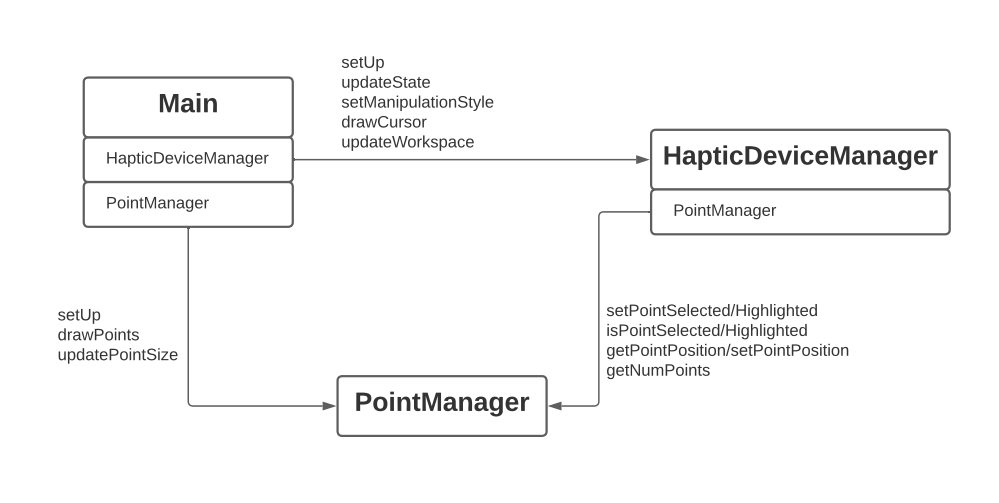
\includegraphics[scale=0.4]{diagrama}

\subsubsection{Guardado de datos}

Para guardar los datos obtenidos de las trayectorias punto\_inicial-punto\_objetivo utilizamos excel. Guardamos los datos en cuatro ficheros diferentes, uno por cada fase del experimento. Cada fichero contiene cinco columnas:
\begin{itemize}
	\item Coordenada x del cursor
	\item Coordenada y del cursor
	\item Número de iteración. Una iteración es un movimiento desde el punto inicial al objetivo.
	\item Punto objetivo. Numerados del 1 al 8.
	\item Tiempo transcurrido desde que se empieza el movimiento, en nanosegundos.
\end{itemize}

Las coordenadas guardadas vienen dadas en coordenadas de pantalla, con respecto a la ventana de visualización donde aparecen los puntos. Para obtener las coordenadas de pantalla a partir de las coordenadas locales, ver sección ...


\subsection{Script en python}

Para poder estudiar los resultados obtenidos implementamos un script en python.

Este script toma los datos de los ficheros excel (utilizando el módulo pandas), y, por cada iteración toma los últimos valores pertenecientes a la posición x, a la posiciçon y y al tiempo. Esto es debido porque queremos quedarnos con la posicion final del cursor. Despues calcula la distancia al punto objetivo de la siguiente manera:

Por ultimo dibuja varias graficas:
\begin{itemize}
	\item Una con la trayectoria realizada entre el punto inicial y el objetivo
	\item Por cada punto objetivo una grafica con los errores cometidos (la distancia desde el ultimo punto al punto objetivo).
	\item Una grafica global con todos los errores cometidos.
	\item Una grafica con el tiempo transcurrido por cada iteracion
\end{itemize}

\section{Obtencion de resultados}

Explicar cómo se han llevado a cabo los experimentos.

\section{Analisis de resultados}


For analysis of hand trajectories, we used Savitzky–Golay
smoothing filter for the measured hand position and velocity.
\chapter{Discusion y conclusiones}


\chapter{Bibliografía}
https://quasardynamics.com/dispositivos-hapticos-la-realidad-virtual/
https://es.3dsystems.com/haptics-devices/touch
\end{document}
